% Created 2025-04-20 Sun 23:21
% Intended LaTeX compiler: pdflatex
\documentclass[11pt]{article}
\usepackage[utf8]{inputenc}
\usepackage[T1]{fontenc}
\usepackage{graphicx}
\usepackage{longtable}
\usepackage{wrapfig}
\usepackage{rotating}
\usepackage[normalem]{ulem}
\usepackage{amsmath}
\usepackage{amssymb}
\usepackage{capt-of}
\usepackage{hyperref}
\usepackage{minted}
\author{Hankertrix}
\date{\today}
\title{Ethics Essay}
\hypersetup{
 pdfauthor={Hankertrix},
 pdftitle={Ethics Essay},
 pdfkeywords={},
 pdfsubject={},
 pdfcreator={Emacs 30.1 (Org mode 9.7.11)}, 
 pdflang={English}}
\usepackage{calc}
\newlength{\cslhangindent}
\setlength{\cslhangindent}{1.5em}
\newlength{\csllabelsep}
\setlength{\csllabelsep}{0.6em}
\newlength{\csllabelwidth}
\setlength{\csllabelwidth}{0.45em * 0}
\newenvironment{cslbibliography}[2] % 1st arg. is hanging-indent, 2nd entry spacing.
 {% By default, paragraphs are not indented.
  \setlength{\parindent}{0pt}
  % Hanging indent is turned on when first argument is 1.
  \ifodd #1
  \let\oldpar\par
  \def\par{\hangindent=\cslhangindent\oldpar}
  \fi
  % Set entry spacing based on the second argument.
  \setlength{\parskip}{\parskip +  #2\baselineskip}
 }%
 {}
\newcommand{\cslblock}[1]{#1\hfill\break}
\newcommand{\cslleftmargin}[1]{\parbox[t]{\csllabelsep + \csllabelwidth}{#1}}
\newcommand{\cslrightinline}[1]
  {\parbox[t]{\linewidth - \csllabelsep - \csllabelwidth}{#1}\break}
\newcommand{\cslindent}[1]{\hspace{\cslhangindent}#1}
\newcommand{\cslbibitem}[2]
  {\leavevmode\vadjust pre{\hypertarget{citeproc_bib_item_#1}{}}#2}
\makeatletter
\newcommand{\cslcitation}[2]
 {\protect\hyper@linkstart{cite}{citeproc_bib_item_#1}#2\hyper@linkend}
\makeatother\begin{document}

\maketitle
\setcounter{tocdepth}{2}
\tableofcontents \clearpage\section{Question}
\label{sec:org4335d30}
The mainstream approaches to normative theory that we have covered in the
second half of the semester include consequentialism, deontology,
and virtue ethics.
Provide an account of a non-mainstream position in normative theory
and offer a critical evaluation of this position with respect to
at least one of the mainstream approaches to normative theory.
\section{Introduction}
\label{sec:org31d9a01}
Mainstream normative theories are filled with flaws
and fail to provide actions that match our intuitions of what should
and should not be done, requiring a lot of modifications to do so,
some of which may do away with core axioms of the theory.

Hence, in this essay, I present an alternative, non-mainstream
normative theory, pragmatic ethics,
which addresses some of the flaws present in
mainstream normative theories.

Let's start with definitions.
Mainstream normative theories are defined as
consequentialism, deontology and virtue ethics.
Normative theory is a framework that establishes standards
or norms for evaluating actions, behaviours and systems.
\section{Overview of pragmatic ethics}
\label{sec:orge75b225}
Pragmatic ethics was developed in response to the dogmatic prescription
of morality by mainstream normative theories.
Instead of identifying an ultimate end or supreme ethical judgement,
pragmatists identify a method for improving our value judgements
(\cslcitation{1}{Anderson, 2005}),
allowing morality to be flexible and responsive to changing environments.
\section{Metaethical concepts of valuing, appraisal and value judgements}
\label{sec:org84f628f}

\subsection{Valuing}
\label{sec:orga3674c9}
A valuing is a tendency towards something,
such as liking or disliking something.
It isn't conscious and has no cognitive value,
and hence is tended to automatically,
without thought or awareness.
An example of a valuing would be Bob liking bubble tea.
\subsection{Appraisal}
\label{sec:orgd90d036}
An appraisal is when a valuing is subjected to questioning, or evaluation.
For example, by asking, "Is it worthwhile to drink bubble tea?"
An appraisal usually occurs when the automatic action on a valuing
is impossible or has adverse consequences.
This is called the problem.
For example, if drinking bubble tea causes stomach ache and diarrhoea
due to lactose intolerance,
should Bob ask for no milk in his bubble tea,
take lactase pills before drinking bubble tea,
or drink bubble tea with plant-based milk?

Alternative solutions and their projected consequences
are generated in the appraisal process,
guiding the formation of a new valuing.
For example, Bob could choose to drink bubble tea without milk,
as taking lactase pills and searching for bubble tea shops
with plant-based milk is too inconvenient.

From the appraisal of the valuing, a value judgement is created,
which in the given example would be "drinking bubble tea without milk
is better than taking lactase pills or searching for bubble tea
with plant-based milk".
This value judgement is practical, as it guides Bob's actions towards
the best solution to his problem.
The valuing generated from the value judgement now has cognitive content,
known as "desire", as the valuing is conscious and is the
result of reflection.
Acting on this new desire results in consequences,
such as experiencing a stronger tea taste,
which goes through the process of appraisal,
creating a new valuing containing greater cognitive content,
and the process repeats.
This results in the refinement of taste.
\subsubsection{Flow chart of the appraisal process}
\label{sec:org3d456d4}
\begin{center}
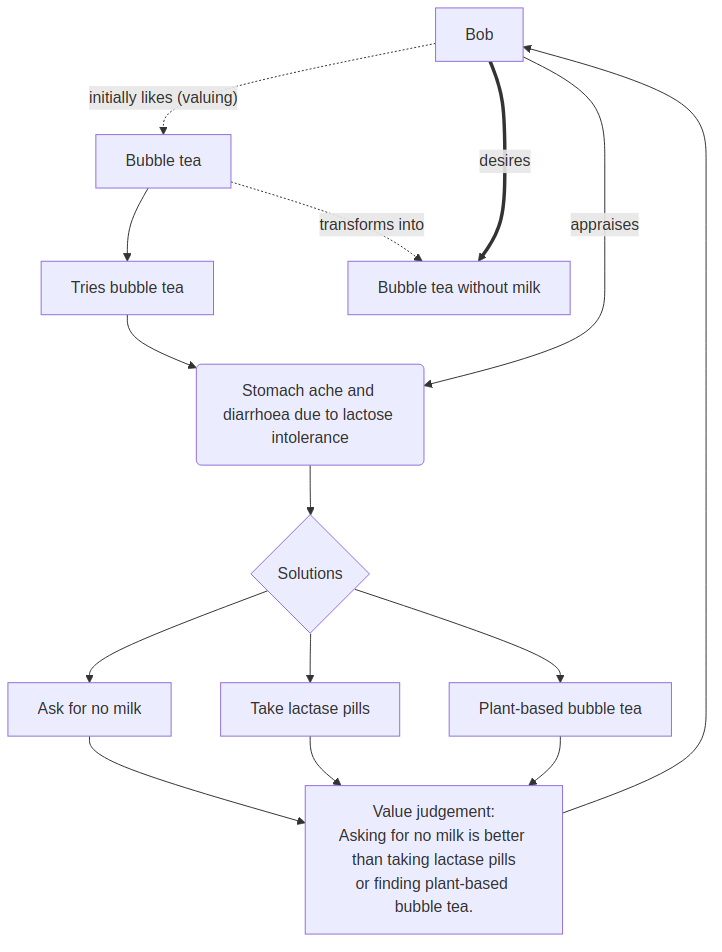
\includegraphics[width=.9\linewidth]{images/appraisal-process.png}
\label{orga723e52}
\end{center}

\clearpage
\subsection{Value judgement as instruments}
\label{sec:orgeb1e13f}
Value judgements are instrumental in 3 ways (\cslcitation{1}{Anderson, 2005}):
\begin{enumerate}
\item Value judgements are practical and action-guiding.
Making them is necessary in deciding on a solution to the faced problem.
\item Value judgements contain the value of actions and objects in
relation to their consequences. They have the form:
if the action is taken, or an object is valued,
then there will be certain consequences, which are valued.
The difference between apparent goods and real goods
is in the valuation of the wider consequences of it,
not just its value when experienced in isolation.
For example, the bubble tea looks good to Bob,
but it isn't actually good after experiencing
stomach ache and diarrhoea after drinking it.
\item Value judgements are tools for discovering how to live a better life,
as cleverly made value judgements are temporary,
and should be changed when the consequences of
acting on them aren't deemed valuable.
\end{enumerate}
\subsection{Empirical validation of value judgements}
\label{sec:org60f8e38}
Since value judgements are instrumental, they can be subjected
to empirical testing and confirmation.
Similar to how scientific hypotheses are tested by bringing
about their antecedents and observing if the results are as predicted,
value judgements can be tested by acting on them
and seeing if the consequences are valued.
Data for validation of a value judgement is generated by acting on it.
A value judgement positing that "basketball is better than soccer"
can be easily tested by trying both sports out and seeing if
there is a preference for one over the other.
\section{Contextualism}
\label{sec:org9cfe1f0}
In pragmatic ethics, contextualism is a moral epistemology
that values the most effective solutions to problems, or what "works".
For example, the most effective solution to Bob's
problem of stomach ache and diarrhoea after consuming
bubble tea is asking for no milk.
Hence, that solution, and the corresponding value judgement,
is considered the most valuable, or "right".

With this epistemology, no action or object has intrinsic value.
Such things have value besides solving a problem,
stripping away the meaning and purpose of value judgements.
\section{Objections}
\label{sec:org98db025}

\subsection{Things are valued as means only}
\label{sec:orgd948d4a}
Contextualism results in value judgements only
containing the value of things as means only,
as things are valued based on their effectiveness
as means to solve a problem.
Ends are neglected in the evaluation of a value judgement,
which are ultimately important.
That means some ultimate end, justified outside of contextualism,
must be given as a standard to evaluate the value of all acts against.
Without it, the justification will fall into infinite regress,
or be justified by our immediate likings,
which is unappealing to most.
\subsection{Descriptive, but not normative}
\label{sec:org92abc29}
Contextualism and value judgements provide a method to determine
"right" actions, but does not provide substantive moral commitments
such as fixed virtues in virtue ethics, moral laws like deontology,
or ultimate ends like the maximisation of the good in consequentialism.
It also depends on the individual's interpretation of what "works"
in a given situation, which suggests the "right" action
may not be the truly "right" action.
Without these commitments, it is difficult
to determine the truly "right" action,
and hence, pragmatic ethics should be relegated
to the realm of metaethics instead of normative theory
due to insufficient action-guidingness.
\section{Response to objections}
\label{sec:org0e5f094}

\subsection{Things are valued as means only}
\label{sec:org6c5e7b8}
Due to the appraisal process,
the value of ends and means is reciprocally determined,
meaning that the value of ends is inextricably tied to
the value of the means to attain it.
In other words, means and ends must be considered as a whole
instead of separate entities.
For example, Bob initially wants to cross a river to see a waterfall,
but after realising that there are no safe ways to cross it,
no longer wants to see the waterfall.
The value of the end (seeing the waterfall) deteriorates
when the consequences of the means (crossing the river)
to attain it are deemed not valuable.
Some valuings are also excluded from the appraisal process,
such as Bob's fear of death, to prevent infinite regress,
but they may be appraised at a later time.
\subsection{Descriptive, but not normative}
\label{sec:org1f3fb8b}

\subsubsection{Collapse argument}
\label{sec:org90ca02a}
Metaethical theories require normative neutrality.
According to LW Sumner,
a metaethical theory that tells us how
moral judgements are justified cannot be morally neutral,
as it would be contradictory
(\cslcitation{2}{Forcehimes, 2015}; \cslcitation{3}{Sumner, 1967}).
Since contextualism tells us how moral judgements are justified,
which is in relation to their consequences,
it is a standard for evaluating actions.
Hence, pragmatic ethics isn't morally neutral,
and collapses to normative theory.
\subsubsection{Pragmatic epistemology}
\label{sec:orgb23a6a3}
Despite being valid, the previous argument
would not appeal to adherents of mainstream normative theories,
as what constitutes the "right" action remains unclear.
Contextualism can be extended with pragmatic epistemology
to result in well-defined "right" actions.

Pragmatic epistemology is based on the central limit theorem,
which states that the distribution of the average of
numerous independent variables to be approximately normal.
This suggests the distribution of value judgements made by
everyone in a situation would be normal,
and converge to a particular judgement, known as the norm.
If this norm persists, it can be considered the "right" action,
because even if every individual value judgement was wrong,
there is a self-norming phenomenon due to the central limit theorem,
and the norm persisting suggests future individuals have
reached similar value judgements.

However, not all norms that emerge as a central tendency are "right",
and not all norms that persist are "right" either.
Hence, some norms will need to be excluded,
similar to how anomalies are excluded from results,
and some value judgements need to be dogmatically normed.
For example, if incest became a norm, it would need to be excluded
as the resulting consequences for humanity are devastating.
Another example is racial harmony being dogmatically normed,
as it improves social cohesion and results in lasting peace.

If the way scientific truths are determined is acceptable,
then the application of pragmatic epistemology for "right" actions
should be acceptable too, as they are the same.
\section{Why pragmatic ethics?}
\label{sec:org61c72f5}
Pragmatic ethics does away with dogma in mainstream normative theories,
making it normatively lean, but allowing flexibility and adaptability
in morality in response to change.
Dogma results in perpetual immaturity,
as moral judgements are fixed, unchanging, and excluded from evaluation,
quickly becoming outdated in rapidly changing circumstances.
Morality becomes stuck in the past, without a way to move forward
or discover a better way to live.

That said, it isn't forbidden to use mainstream normative theories
as justification in pragmatic ethics, but instead of treating them
as the only way of justification, they are treated as hypotheses
to be empirically validated in practice through the appraisal process.
Any other normative theories, like casuistry,
can be used as justification,
so long as the resulting action resolves the problem at hand.
\subsection{Against consequentialism}
\label{sec:org2ee454a}
Imagine the situation of a wife and a minister in a burning building,
and the husband only being able to save one of them.
Standard agent-neutral consequentialism
will recommend that the husband save the minister,
as saving the minister maximises the good.
This does not line up with the husband's intuition,
as most would save their wife instead.

To resolve this discrepancy, the agent-neutral axiom of consequentialism
is forgone and an obligation to prefer friends and family is introduced.
The core consequentialist commitment
of maximising the good is hence violated in some situations,
resulting in moral schizophrenia,
which is when one's motives and justifications are not aligned.

In contrast, pragmatic ethics has no such issue.
The solution that "works" is for the husband to save his wife,
and the same goes for the moral norm,
hence there is no conflict with our intuitions.
Pragmatic ethics would never conflict with our intuitions,
as the "right" action is always empirically determined.

\clearpage
\subsection{Against deontology}
\label{sec:orgdcaf1d3}
Deontology uses fixed rules and duties to determine the "right" action.
These will ultimately become outdated and irrelevant
from their inability to be updated.
For most divine command theorists,
these rules and duties are taken from religious texts
written thousands of years ago.
Some of which are no longer applicable in modern times,
such as Leviticus 20:13 stating homosexuality is punishable by death.

Rules that aren't concretely defined still face the same issue.
The categorical imperative in Kantian ethics states,
"Act only in accordance with that maxim that
you can at the same time will that it become universal law."
Any action resulting in a contradiction when universalised,
such as killing for pleasure, violates the categorical imperative,
and is considered immoral.
However, even moral maxims can violate the categorical imperative.
For example, if everyone helps the poor,
there will be no poor people to help, resulting in a contradiction.
Thus, helping poor people is considered immoral.
Immoral maxims can pass the categorical imperative too,
like keeping all promises except one.
Since these rules cannot be changed,
they will forever remain outdated
and require exceptions and additional circumstantial rules
to be bolted on to match our intuitions,
increasing the complexity of the theory,
and making it more difficult for the layman to use.

Conversely, pragmatic ethics has a simple procedure and is flexible,
allowing it to stay up-to-date and adapt with the times
to always match our intuitions.
Exceptions and circumstantial rules aren't required,
ensuring that pragmatic ethics remains
simple and accessible to the layman.
\section{References}
\label{sec:org85f2c8e}
\begin{cslbibliography}{1}{0}
\cslbibitem{1}{Anderson, E. (2005). \textit{Dewey’s moral philosophy}.}

\cslbibitem{2}{Forcehimes, A. T. (2015). On lw sumner’s “normative ethics and metaethics”. \textit{Ethics}, \textit{125}(4), 1142–1144.}

\cslbibitem{3}{Sumner, L. W. (1967). Normative ethics and metaethics. \textit{Ethics}, \textit{77}(2), 95–106.}

\end{cslbibliography}
\end{document}
